\documentclass[10pt,letterpaper]{article}
\usepackage{amsmath}
\usepackage{amssymb}
\usepackage{fancyhdr}
\usepackage[bottom=1in, top=1in, left=1in, right=1in]{geometry}
\usepackage{graphicx}
\usepackage{here}
\usepackage{subfigure}
\usepackage[T1]{fontenc}
\DeclareGraphicsExtensions{.pdf,.png,.jpg}

\pagestyle{fancy}
\setlength{\headheight}{.5in}
\setlength{\parindent}{0in}

\begin{document}

\rhead{
          Paul Boschert\\
          09/11/2015\\
          CSCI 5622 - Machine Learning: Homework 2 Analysis \\
      }


\textbf{\textit{1)}} The role of the learning rate is to more quickly (or more slowly) get to an optimal solution.  It controls the magnitude of the changes to the $\beta_{j}$ values.  A step size, $\lambda$, that is too large can quickly cause the exp() function to overflow because it may create very large $\beta_j$ values.\\
\begin{equation}
  \pi_{i} = \frac{e^{\beta^{T}x_i}}{1 + e^{\beta^{T}x_i}}
\end{equation}
Generally speaking, the learning rate is usually chosen by trial and error.  If it's not constant, it usually gradually decreases as the iteration number increases.\\

\textbf{\textit{2)}} With a constant step size of one, the accuracy of the training data and the test data start to level out around iteration $\sim800$.  See Figure \ref{fig:accuracyVsIteration} for more details.\\
\begin{figure}[ht]
  \centering
  \subfigure[The relationship of accuracy and iteration]{
    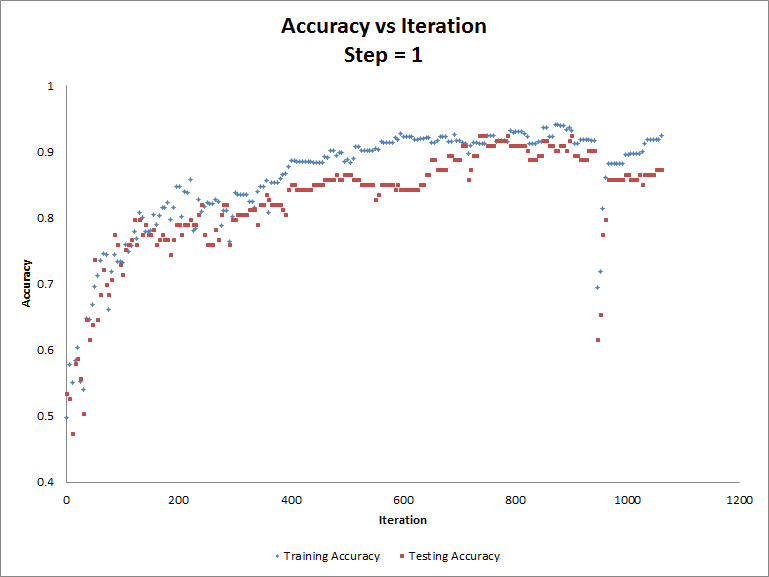
\includegraphics[scale=.35]{accuracyVsIteration}
    \label{fig:accuracyVsIteration}
  }
  \subfigure[The relationship of accuracy and iteration different steps]{
    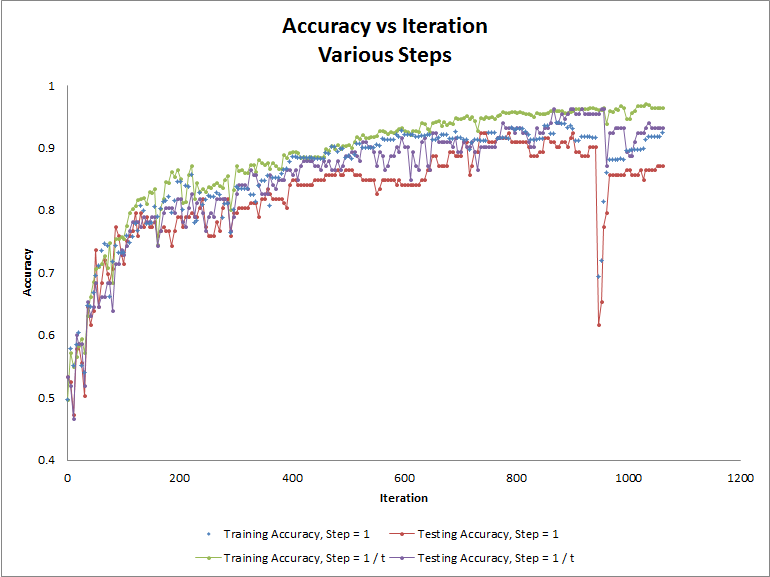
\includegraphics[scale=.35]{accuracyVsIterationStep1}
    \label{fig:accuracyVsIterationStep1}
  }
  \caption{Accuracy and learning rate}
  \label{fig:figure}
\end{figure}

\textbf{\textit{3)}} The words that are the best predictors have the largest $|\beta_{j}|$ values.  I sorted the final $\beta$ array using numpy.argsort.  This gives back indices that would sort the array.  Then I used the last five indices and the first five indices to index into the vocab array to get the words.  The first five (greatest negative values) are associated with the Hockey classification, and the last five (greatest positive values) are associated with the Baseball classification.  An important note here: I used the entire data set, and I also used a $\lambda_t = 1 / t$ where $t$ is the iteration.
The five best predictors are:\\
\begin{tabular}{c|l|c||l|c}
  & \multicolumn{2}{|c||}{Hockey} & \multicolumn{2}{c}{Baseball}\\
  \hline
  Num & Word & $\beta$ & Word & $\beta$\\
  \hline
  0 & hockey & -1.851942 & hit & 1.207308\\
  1 & playoffs & -1.270941 & runs & 1.146263\\
  2 & pick & -0.995942 & bat & 0.929948\\
  3 & playoff & -0.904541 & saves & 0.900354\\
  4 & points & -0.901229 & pitching & 0.840741\\
\end{tabular}
\\
\\

\textbf{\textit{4)}} The words that are the worst predictors have the smallest $|\beta_{j}|$ values.  I sorted the final $\beta$ array using numpy.argsort.  This gives back indices that would sort the array.  Then I looped through the array until I saw a sign change which indicates a change in classification for either the Hockey classification or the Baseball classification.  Once I saw a change in sign, I walked back five values to find the worst predictors for the Hockey classification, and I walked forward five values to find the worst predictors for the Baseball classification.  I used these indices to index into the vocab array to get the words.  An important note here: I used a $\lambda_t = 1 / t$ where $t$ is the iteration.  Another potential ambiguity: some might argue that the worst predictors for a particular classification are the best predictors for a different classfication for example a $\beta_j = 2$ is so far away from the Hockey classification that it's the worst predictor.  I did not do this, I chose to interpret the question to mean that we should find the worst predictors for a particular classification that still actually predict that classification.
The five worst predictors are:\\
\begin{tabular}{c|l|c||l|c}
  & \multicolumn{2}{|c||}{Hockey} & \multicolumn{2}{c}{Baseball}\\
  \hline
  Num & Word & $\beta$ & Word & $\beta$\\
  \hline
  0 & silence & 0.000000 & tandem & 6.43996e-13\\
  1 & everywhere & 0.000000 & terrific & 6.43996e-13\\
  2 & riel & 0.000000 & partly & 7.89948e-13\\
  3 & intermissions & 0.000000 & chicago & 2.00711e-12\\
  4 & tone & 0.000000 & dive & 2.00711e-12\\
\end{tabular}
\\
I belive the values for Hockey are 0 instead of slightly negative because of the precision available.  Those values do indicate a different sign because that's how I found them, but when printed out they are so small, they show zero.
\\

\textbf{\textit{EC 1)}} At first I attempted to use a variable learning rate that was simply $1 / t$.   The effect was generally better.  See Figure \ref{fig:accuracyVsIterationStep1}
Then, I looked at the scikit-learn python package.  When the learning rate is set to `optimal' it is implemented as $\lambda_{t} = \frac{1}{\alpha(t_0 + t))}$
Where $t_0$ is chosen heuristically using a method proposed by L\'eon Bottou.  After reading the relevant sections of his paper \cite{sgdpaper}.  I tried using a smaller data set to determine the optimal $\gamma_0$ value from the formula given in \cite{sgdpaper}, $\gamma_t = \gamma_{0}(1 + \gamma_{0}\lambda t)^{-1}$.  Unfortunately, this gave me nearly identical results to $\lambda_t = 1 / t$.


\begin{thebibliography}{1}
  \bibitem{sgdpaper} Bottou, L\'eon {\em Stochastic Gradient Descent Tricks,  http://research.microsoft.com/pubs/192769/tricks-2012.pdf}, 2012. PDF file.
\end{thebibliography}

\end{document}

